\documentclass{beamer}
\usepackage[utf8]{inputenc}
\usepackage{subfiles}
\usepackage{lipsum}
\usepackage{float}
\usepackage{listings}
\usepackage{color}
\usepackage{tikz}
\usepackage{lmodern}

\definecolor{darkblue}{rgb}{0.086,0.145,0.357}
\definecolor{darkpurple}{rgb}{0.3098,0 , 0.3098}
\definecolor{skinorange}{rgb}{0.957,0.639 , 0.365}


\usetikzlibrary{arrows.meta,arrows}
\usetikzlibrary{positioning}

\usetheme{Madrid}
\usecolortheme{beaver}

\title[About Beamer]{Priority Queue}
\subtitle{An Introduction}

\author[A.A. and A.N.F]{Md Awsaf Alam \inst{1} \\ Ahmed Nafis Fuad\inst{2}}

\institute{
\inst{1}
Department of CSE\\
BUET\\
\inst{2}
Department of CSE\\
BUET
}

\date{\today}

\AtBeginSection[]{
\begin{frame}{We are going to see}
    \tableofcontents[currentsection]
\end{frame}
}

\begin{document}
\titlepage

\begin{frame}{Table of Contents}
\tableofcontents

\end{frame}
\section{Introduction}

\begin{frame}

\frametitle{Sample Frame}
A Binary (Max) Heap is a complete binary tree that maintains the Max Heap property.

Binary Heap is one possible data structure to model an efficient Priority Queue (PQ) Abstract Data Type (ADT). In a PQ, each element has a "priority" and an element with higher priority is served before an element with lower priority (ties are broken with standard First-In First-Out (FIFO) rule as with normal Queue). Try clicking ExtractMax() for a sample animation on extracting the max value of random Binary Heap above.

To focus the discussion scope, we design this visualization to show a Binary Max Heap that contains distinct integers only.

\end{frame}

\section{Problem Definition}
\begin{frame}{Simulation}

\end{frame}


\begin{frame}{Another Simulation}
\setbeamercovered{dynamic}
\begin{center}
  \begin{tabular}{|c|c|c|}
      \hline
      Table & X & Y\\
      \hline
      A & \onslide<1->{1} & \onslide<2->{0}  \\
      \hline
      B & \onslide<3->{0} & \onslide<4->{1}  \\
      \hline
  \end{tabular}
\end{center}

\end{frame}


\section{Motivation}

\begin{frame}{Use of Columns and Images}
\setbeamercovered{dynamic}  % Ghola korar jonno

  \begin{columns}
    \column{0.5\textwidth}

    \begin{figure}[H]
        \centering
        \label{fig:2}
        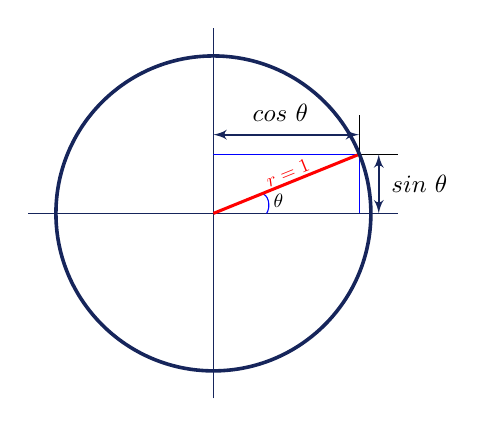
\begin{tikzpicture}[scale=0.5]

           \draw [darkblue,line width= 0.5pt] (-4.7,0) -- (4.7,0);
           \draw [darkblue,line width= 0.5pt] (0,-4.7) -- (0,4.7);

           \draw [blue] (0,1.5) -- (3.7,1.5);
           \draw [darkblue,line width= 0.7pt,{latex'[width= 5pt, length=5pt]}-{latex'[width= 5mm, length=5mm]}] (0,2) -- (3.7,2);
           \node [scale = 0.9pt, above] at (1.7 , 2.1){$cos ~\theta$};

           \draw (3.7,1.5) -- (4.7,1.5);

           \draw [blue] (3.7,0) -- (3.7,1.5);
           \draw [darkblue,line width= 0.7pt,{latex'[width= 5pt, length=5pt]}-{latex'[width= 5mm, length=5mm]}] (4.2,0) -- (4.2,1.5);
           \node [scale = 0.9pt, right] at (4.3, 0.75){$sin ~\theta$};

           \draw (3.7,1.5) -- (3.7,2.5);

           \draw [blue](1.35 , 0) to [in=5,out=55] (1.2, 0.50);
           \node [scale = 0.7pt ,above] at (1.65, -0.02){$\theta$};

           \draw [red,line width= 1.1pt] (0,0) -- (3.7,1.5);
          \node [scale = 0.7pt,red,rotate = 22 ,right] at (1.2, 0.75){$r = 1$};

          \draw[darkblue,line width= 1.3pt] (0,0) circle (4);

        \end{tikzpicture}

        \caption{Alternate representation of Pythagorean theorem.}
    \end{figure}

    \column{0.5\textwidth}

    \includegraphics[height=1.6cm]{tree.png}
    \end{columns}

\end{frame}

\section{Design}

\section{Previous Works}
\begin{frame}{Blocks}
    \begin{block}{Sample Block}
    This is a sample block.
    \end{block}
    \begin{alertblock}{Sample Alert Block}
    This is a sample \textbf<2>{alert block}.
    \end{alertblock}
    \begin{example}
    Sample \textcolor<3->{red}{example}.
    \end{example}
\end{frame}
\section{Conclusion}


\end{document}
\begin{frame}{Use of Columns and Images}
    COncluded
\end{frame}
